\chapter{博洛尼亚美院入学指南}              


\section{博洛尼亚美术学院简介}
博洛尼亚美术学院(Accademia di Belle Arti di Bologna也称Accademia Clementina)。\\
在1711年10月由十一世教皇Clemente XI 签署文件成立,至今已有300余载。美院座落于博洛尼亚古城内,地址:Via Belle Arti, 54.

\subsection{院系}
美院分为四大院系,分别为:

\begin{itemize}
\item 视觉艺术系(Dipartimento Di Arti Visive)
\item 应用艺术与设计系(Dipartimento Di Progettazione Ed Arti Applicate)
\item 文物修复系(Dipartimento Di Restauro)
\item 艺术教育与传播系(Dipartimento Di Comunicazione E Didattica Dell’Arte)
\end{itemize}

\subsection{学位专业}

\subsubsection{本科}
三年制本科共开设11个专业,分别为:舞台美术(Scenografia),电视电影摄影(Fotografia cinema e televisione),绘画(Pittura),雕塑(Scultura),产品设计(Design di prodotto),服装设计(Fashion design),装饰环境与艺术(Decorazione indirizzo arte e ambiente),版画(Grafica d’arte),平面设计(Design grafico),漫画与插画(Fumetto e illustrazione),艺术教育与传播(Didattica e comunicazione dell’arte)。
      
\subsubsection{硕士}
两年制硕士共开设12个专业,分别为:雕塑(Scultura),绘画(Pittura),服装设计(Fashion design),摄影(Fotografia),建筑装饰(Decorazione per l’architettura),版画(Grafica d’arte),插画(Illustrazione per l’editoria),漫画语言(Linguaggi del fumetto),电视电影(Cinema e Televisione),舞台美术(歌剧方向,Cesena校区)(Scenografia del melodramma e del teatro musicale),舞台美术(展览方向)(Scenografia e allestimenti),文化艺术遗产与教学(Didattica dell’arte e mediazione culturale del patrimonio artistico)。


\section{博洛尼亚美术学院入学考试注册说明}
\textbf{第一步:邮局缴费}\\
在邮局Poste拿叫做1016的小条,缴费16.13欧。(记得打印)\\

\textbf{第二步:考试缴费}\\
学校账号:IT14 T062 7013 199T 2099 0000 640  (La Cassa di Ravenna S.p.A, CODICE BIC/SWIFT: CRRAIT2RXXX)\\
缴费给intestato a: Accademia di Belle Arti di Bologna \\
缴费原因causale: Contributo prova di ammissione\\
(考试费为一门50欧,最多可报三门,第三门缴费30欧。)\\

\textbf{第三步:进入网站}\\
https://www.servizi2.isidata.net/SSdidatticheac/MainGenerale.aspx?lng=it-IT\\
此网页为各大美院注册个人信息网站,也可以扫描下方二维码访问\\
\\
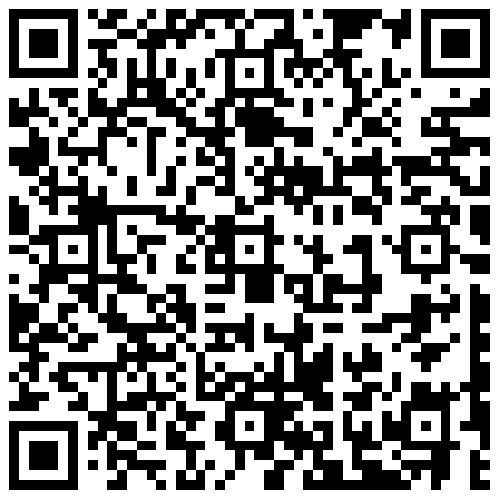
\includegraphics[scale=0.3]{ababoqrcode}\\

\textbf{第四步:申请账户}\\
点击申请账户:Inserimento domanda di AMMISSIONE\\
找到更改信息和打印申请表:ModificaStampa domanda di AMMISSIONE,点击。\\
选择Seleziona l’Accademia,选择 BOLOGNA。\\

\textbf{第五步:填表并上交}\\
跳出表格后进行填写。(带*的是必填的)\\
CORSO 下拉栏显示的是要注册的专业,本科专业是以(TRIENNIO)结尾的,研究生专业以(BIENNIO)结尾。\\
填写完后点击提交。(上传后有账号和密码,建议截图保存)\\

\textbf{第六步:上传缴费单}\\
找到tasse按钮,选择inserisci una nuova tassa。\\
点击“选择文件”上传缴费单。(文件小于2M)\\
(注意拍照清晰,文件为秘书处人工审查)\\
最后点击(inserisci)上传。\\

\textbf{第七步:上传所有材料}\\
包括所有在大使馆认证的材料以及护照和居留的电子版。\\
点击左上角的 allega documentazione,来上传自己的所有文件(文件小于2M)\\
(一旦正式确定提交,就不能再更改了!!!)\\
点击提交按钮INVIA DOMANDA\\

\textbf{附材料列表:}\\
\begin{itemize}
\item dati anagrafici  个人资料
\item recapito telefonico/e-mail  电话号码/电子邮件地址
\item permesso/carta di soggiorno valido o copia della ricevuta attestante la richiesta  居留/有效的居留或收据证明副本;
\item dichiarazione di valore in loco attestante il conseguimento del titolo finale degli studi secondari e il del Diploma Accademico di 1° livello o di Laurea prevista per l’accesso all’Università 价值证明
\item titolo con relativa traduzione ufficiale 翻译文件
\item domanda di preiscrizione presso l’ambasciata大使馆预注册文件;
\item permesso/carta di soggiorno valido o copia della ricevuta attestante la richiesta  居留/有效的居留或收据证明副本;
\item autenticazione di fotografia rilasciata dalla rappresentanza diplomatica italiana all’atto della preiscrizione.在预注册时由意大利使馆代表签发的照片鉴定。

\end{itemize}


\textbf{第八步:检查}\\
https://www.servizi2.isidata.net/SSdidatticheac/MainGenerale.aspx?lng=it-IT\\
进入该网站,点击第二个更改信息ModificaStampa domanda di AMMISSIONE。(anche per iscrizione diretta - senza esame di ammissione)\\
选择学校,填写邮箱收到的账号密码,点击提交信息INVIA DOMANDA。\\
进入页面后可以看到一张图,绿色的表示上传成功,红色的表示缺少材料。\\
最后点击下方的按钮—conferma i dati ed invia la domanda完成提交。\\
\\
注意:提交之后不能更改,如果之后发现邮箱等信息错误,只能去秘书处现场更改。\\
\\
\section{参加入学考试}

\subsection{考试内容}
1、意大利语考试。博洛尼亚美术学院每年会单独组织 B2 等级的意大利语考试,所有考生必须通过该考试才能够参加专业考试。考试内容大致为语法以及艺术历史相关知识\\
2、专业考试。美院各专业会分别单独举行专业考试,考试时间及考试地点请登陆美院官网查询:www.ababo.it/ABA/ammissioni-on-line,考试内容及更多详细信息请联系美院学联:segreteria.usscababo@gmail.com

\subsection{考试结果查询}
语言考试结果会在一周之内在美院官网首页公布:www.ababo.it\\
专业考试结果会在专业考试结束之后一周内分别在美院官网首页公布。(所有专业考试结束之后,未报满的专业有可能会有补考机会,请持续关注美院官网)\\

\section{正式注册入学}

通过专业考试的新生必须在学校规定时间内进行正式注册。正式注册所需材料为:重要提醒:材料尽量只提交复印件,保留原件,如遇必要情况也请同学们做好备份\\
\begin{itemize}
\item 新生注册申请表一份(http://www.ababo.it/ABA/iscrizioni/)
\item 护照复印件
\item 两张两寸白底证件照
\item 税费1,€102.94,邮局索取 1016 号汇款单,填写格式参考报名税
\item 税费2,€140,邮局索取普通三联汇款单并填写:c/cp.n:68882703,intestato a :Regione Emilia Romagna,causale: Tassa diritto allo studio universitario a.a. XX/XX(学年)
\item 分级缴费,需要提交 ISEE 证明。\\
需上传缴费单到 (https://www.servizi.isidata.it)等秘书处确认。到任意银行汇款至美院账户:c/c bancario IT76 K070 7202 4040 9000 0178 822 (Emil Banca)intestato all’Accademia di Belle Arti di Bologna, causale“prima rata a.a.XX/XX(学年)
\item permesso/carta di soggiorno valido o copia della ricevuta attestante la richiesta  居留/有效的居留或收据证明副本;
\item autenticazione di fotografia rilasciata dalla rappresentanza diplomatica italiana all’atto della preiscrizione.在预注册时由意大利使馆代表签发的照片鉴定。
\\
\end{itemize}
将缴费收据同其他材料在截止日期前一并在线上传,不需要邮寄。\\
https://www.servizi.isidata.it

\section{美院地图}
(可关注学联公众号“博洛尼亚美院学联ASSCABO”查看)
\subsection{上课时间及安排}
各专业的课表(piano di studio)在此查询:www.ababo.it/ABA/piani-di-studio-anno-corrente/ 
各专业具体上课时间,地点及授课教授安排(orari corsi),在此查询:www.ababo.it/ABA/orari-corsi/
开学第一周每门课程的教授都会开设课程介绍,如有多名教授同时开设同一门课程,可任选一个教授直接去上课即可。
\subsubsection{选课,课表提交及workshop}
查看课表(piano di studio),不同专业会安排不同选择范围的选修课(Attività formative a scelta dello student), 不同专业可选范围不同,请在各专业可选范围内选择,选择好之后需填写课表提交申请并由各专业负责教授(coordinator)签字,并在截止日期之前进行复印投至系办公室门口信箱,信箱位于I2教室走廊中间,截止日期,可选范围及课表提交申请详情及下载链接参考美院官网:http://www.ababo.it/ABA/modulistica-studenti/
workshop的不同课程所安排及所给学分不同,workshop课程预告会在美院官网首页公告栏和校内张贴公告,请大家详细阅读课程安排以及学分安排,如有报名要求需提前报名确认。上完workshop课程结束之后需向教授要结课证明,填写对应学分并由教授签字,进行复印并投至系办公室门口信箱。
\subsubsection{workshop学分获取说明}
本科三年制共180学分,研究生两年制共120学分。其中一项为「额外的培训活动」Attivita formative ulteriori,其中包括Workshop,Seminari,tirocini等形式。
Workshop一般是指有固定主题的实践课程。学生们在教授的带领下,通过教授的指导和示范,最终会做出一些作品,比如:装置,绘画,模型等等。根据美院专业的不同,需要获取的学分也不同,学生需要修满此项学分才可以顺利毕业。通过参加不同主题的workshop,在获取学分的同时,也可以学到很多实用有趣的技能。
Workshop的时间、地点、主题可以通过美院的官网进行了解。参与学校或是教授组织的活动需要留意美院官网信息与对应教授进行沟通参加。
\subsubsection{学生卡、学生手册及居留证明}
学生卡为学生的身份证明,学生手册(libretto d’iscrizione),大约会在开学之后一个月时间左右在官网发出通知,学生需携带有效证件前往美院秘书处领取。
学生手册非常重要,缴纳学费之后需本人拿到美院秘书处盖章(timbrare),每次考试必须携带,考试之后教授会在上面登记成绩并签字,此次考试方可生效。
续居留所需的学校证明现在都是学生自己打印 (https://www.servizi.isidata.it) 无需学校盖章。如特殊情况,需正式在读证明,需要2张marca da pollo交于秘书处。
\subsubsection{考试流程}
每年学校将会安排三次考试季,分别为: 夏季 (6-7 月),秋季 (9-10月), 补考季 (2-3月)。
考试季为网上预约 (https://www.servizi.isidata.it),错过预约不能参加考试。
\subsubsection{老生新学期注册}
美院老生注册,按照教程进行注册并打印,随同缴费单一起 交至美院秘书处。\\
教程地址:http://www.ababo.it/ABA/wpcontent/uploads/2011/07/ESEMPIO-ISCRIZIONI-ON-LINE2012-131.pdf tassa di frequenza
可申请减免,减免要求:上 一学年考试通过五门考试,并且每门考试分数在 24/30 分以 上 (包括 24 分),填写减免申请表并提交至美院秘书处,申请表下载地址:http://www.ababo.it/ABA/iscrizioni/
\subsubsection{ER-GO奖学金学分要求}
ER-GO奖学金对博洛尼亚美院的学分要求为:本科,研究生五年制本硕连读:第一学年结束需修满40学分,第二学年结束需修满90学分,本科及五年制本硕连读第三学年结束需修满135学分。
学分需在每年夏季考试结束之前(八月份)修满方可达到奖学金发放要求并满足申请下学年奖学金申请条件。如未修满,可申请借分(BONUS),第一年可借:5学分,第二年可借:12学分,第三年可借:15学分,借分要求及使用方法请咨询ER-GO官方,详情请查寻ER-GO官网:http://www.er-go.it/

\section{毕业相关}
博洛尼亚美院每年会有三次毕业季,分别在三次考试季之后,毕业流程分为三步:

\subsubsection{第一步:提交毕业申请表}
学生可在剩余两门课程学分未修满并确保毕业答辩之前可修满的情况下提交毕业申请表,各系需填写相对应申请表,申请表需指导教授及本人签字并投至系办公室门口信箱,申请表下载地址:http://www.ababo.it/ABA/tesi/,截止日期(2015年)分别为:

\begin{itemize}
  \item 夏季毕业:2015年3月16日之前
  \item 秋季毕业:2015年7月13日之前
  \item 期外毕业:2015年12月4日之前
\end{itemize}

\subsubsection{第二步:提交毕业所需材料}
需提交材料为:
\begin{itemize}
  \item 学生手册
  \item 毕业论文电子版CD(封面需按照要求打印并有论文指导教授签字)(Allegato 6)
  \item Allegato 4
  \item Marca da bollo€16
  \item 邮局汇款€90.84至1016号账户,并提交收据
  \item A4纸大小信封,附上€2.4邮票,并在信封上填写有效家庭住址,将用于接收毕业证明
\end{itemize}
论文封面请按照正规格式排版,参考Allegato 5。所有表格及当年毕业详细信息在美院官网毕业专区内名为NORME PRESENTAZIONE TESI的PDF文件中。


\subsubsection{第三步:毕业答辩}
答辩需准备装订成册的正式毕业论文,前往规定时间和地点参加答辩。美院官网会发布毕业答辩时间安排,最新信息请关注美院官网毕业专区:http://www.ababo.it/ABA/tesi/\\

\section{博美中国学联简介}
博洛尼亚美术学院中国学联 (Unione degli Studenti e Studiosi Cinesi al Accademia di Belle Arti Bologna) 是一个在罗马教育处注册过的合法的,非营利性,非政治性的学生团体,作为公益性社团组织,博美中国学联致力于:
\begin{itemize}
  \item 在美院范围内促进各专业之间的联系、交流与合作
  \item 立足于服务中国留意学者学生的学习、生活和工作,促进专业学术研讨
  \item 维护中国留意学者学生在意的合法权益
  \item 通过开展和参与形式多样的文体活动、推动留意学者学生与意大利社会各界、中国国内以及华人国际社会的联系和交流,促进中意两国互动与交流
\end{itemize}

博美中国学联由以下部门组成:秘书处,外联部,宣传部,组织部。欢迎广大同学积极参与。\\
加入学联方式:seg.asscabo@gmail.com\\
微信公众号平台“博洛尼亚美院学联ASSCABO”\\


